\chapter{Mantle as a File System Metadata Load Balancer}
\label{mantle}

%%%%%%%%%%%%%%%%%%%%%%%%%%%%%%%%%%%%%%%%%%%%%%%%%%%%%%%%%%%%%%%%%%
\section{Introduction}								    %%%%%%%%%%
\label{introduction}								    %%%%%%%%%%
%%%%%%%%%%%%%%%%%%%%%%%%%%%%%%%%%%%%%%%%%%%%%%%%%%%%%%%%%%%%%%%%%%
% What is the metadata management problem?


Accessing metadata is a bottleneck for large file systems. Single disk POSIX
file systems consult metadata before seeking to the data. First they translate
the file name into an inode. Then they use that inode to lookup their metadata
in an inode table, which is at some fixed location on disk. 

Serving metadata and maintaining a POSIX namespace is challenging for
large-scale distributed file systems because accessing metadata imposes small
and frequent requests on the underlying storage
system~\cite{roselli:atec2000-FS-workloads}. As a result of this skewed
workload, serving metadata requests does not scale for sufficiently large
systems in the same way that read and write throughput
do~\cite{abad:ucc2012-mimesis, alam:pdsw2011-metadata-scaling,
weil:osdi2006-ceph}. Many distributed file systems decouple metadata from data
access so that data and metadata I/O can scale
independently~\cite{alam:pdsw2011-metadata-scaling, ghemawat:sosp2003-gfs,
hildebrand:msst2005-pnfs,weil:osdi2006-ceph,welch:fast2008-panasas,xing:sc2009-skyfs}.
These ``metadata services" manage the namespace hierarchy and metadata requests
({\it e.g.}, file and directory creates, file and directory renaming, directory
listings). File properties that a metadata service manages can include
permissions, size, modification times, link count, and data location. 

%konstantinos:pdsw2014-lustre-metadata

\begin{figure}[tb]
	\centering	
	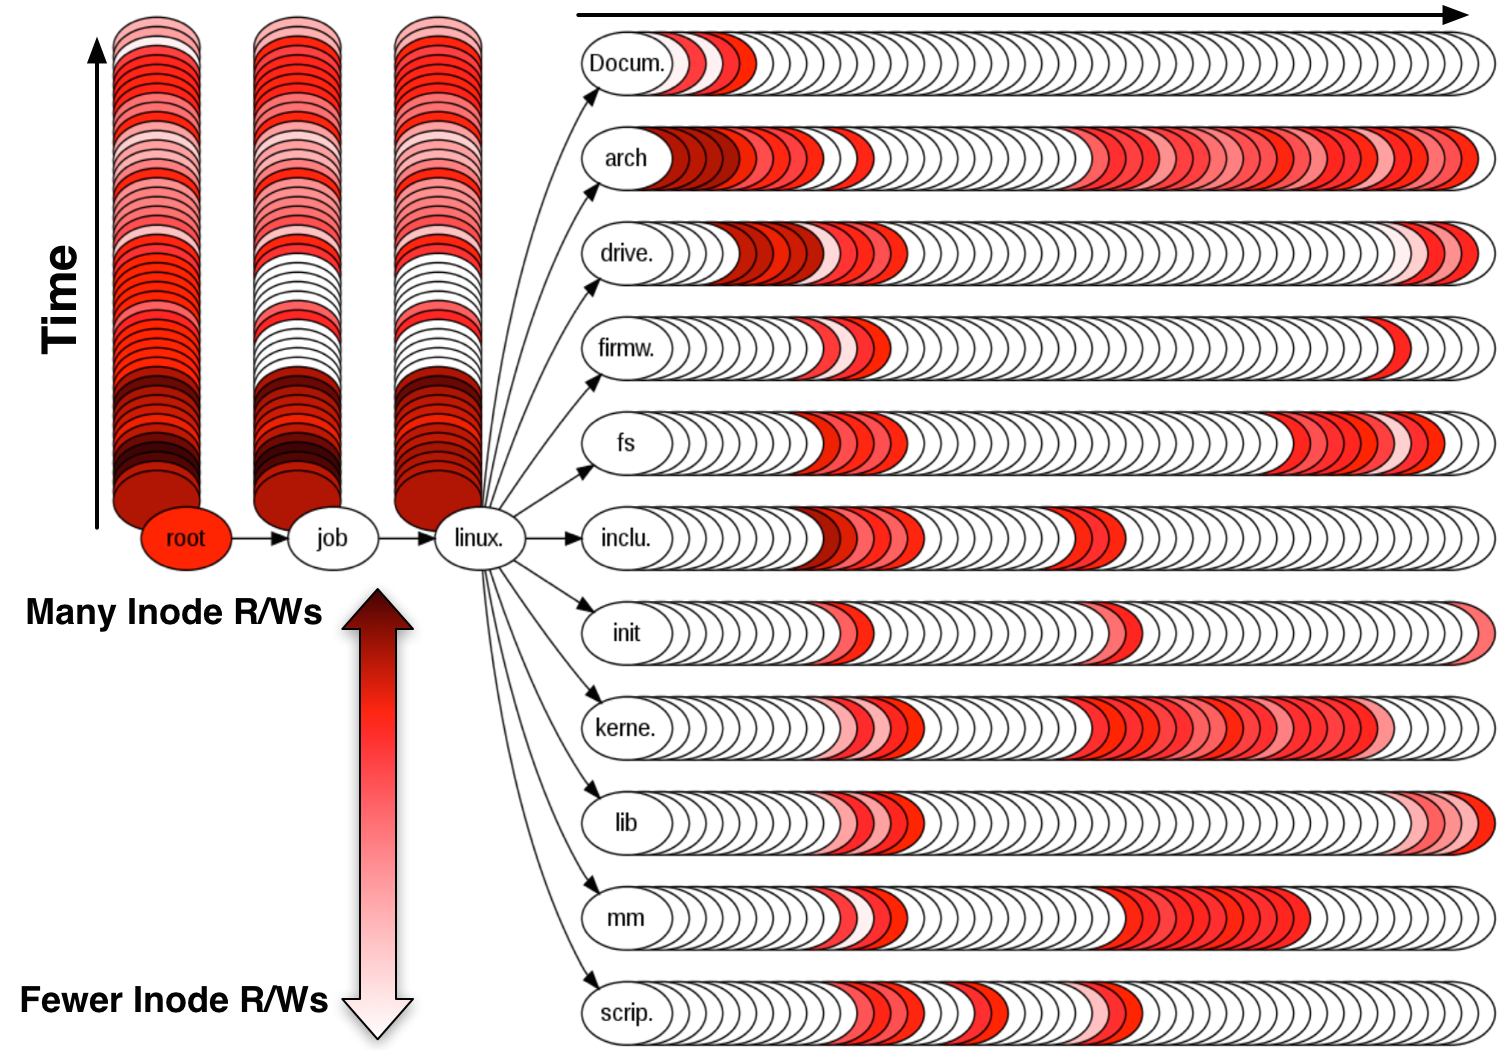
\includegraphics[width=0.5\textwidth]{./chapters/mantle/figures/workload-tar.png}
	\caption{Metadata hotspots, represented by different shades of red, have spatial and temporal locality when compiling the Linux source code. The hotspots are calculated using the number of inode reads/writes and smoothed with an exponential decay. \label{figure:workload-tar}}
\end{figure}

% Why you should care: metadata management as a resurgence
Unfortunately, decoupling metadata and data is insufficient for scaling and many setups require customized application solutions for dealing with metadata intensive workloads. For example, Google has acknowledged a strain on their own metadata services because their workloads involve many small files ({\it e.g.}, log processing) and simultaneous clients ({\it e.g.}, MapReduce jobs)~\cite{mckusick:acm2010-gfs-evolution}. Metadata inefficiencies have also plagued Facebook; they migrated away from file systems for photos~\cite{beaver:osdi2010-haystack} and aggressively concatenate and compress small files so that their Hive queries do not overload the HDFS namenode~\cite{thusoo:sigmod2010-facebook-infrastructure}. The elegance and simplicity of the solutions stem from a thorough understanding of the workloads ({\it e.g.}, temperature zones at Facebook~\cite{muralidhar:osdi2014-f4}) and are not applicable for general purpose storage systems. 

% Multi-MDS problem: synchronizing access and coalescing knowledge 
The most common technique for improving the performance of these metadata services is to balance the load across dedicated metadata server (MDS) nodes~\cite{patil:fast2011-giga+,weil:osdi2006-ceph,weil:sc2004-dyn-metadata,sinnamohideen:atc2010-ursa,xing:sc2009-skyfs}. Distributed MDS services focus on parallelizing work and synchronizing access to the metadata. A popular approach is to encourage independent growth and reduce communication, using techniques like lazy client and MDS synchronization~\cite{patil:fast2011-giga+, ren:sc2014-indexfs, zheng:pdsw2014-batchfs, hildebrand:msst2005-pnfs, zhu:pds2008-hba}, inode path/permission caching~\cite{brandt:mss2003-lh, li:msst2006-dynamic, xing:sc2009-skyfs}, locality-aware/inter-object transactions~\cite{sinnamohideen:atc2010-ursa,zhu:pds2008-hba,ren:atc2013-tablefs, ren:sc2014-indexfs} and efficient lookup tables~\cite{brandt:mss2003-lh, zhu:pds2008-hba}. Despite having mechanisms for migrating metadata, like locking~\cite{sinnamohideen:atc2010-ursa,schmuck:fast2002-gpfs}, zero copying and two-phase commits~\cite{sinnamohideen:atc2010-ursa}, and directory partitioning~\cite{xing:sc2009-skyfs, patil:fast2011-giga+, ren:sc2014-indexfs, weil:osdi2006-ceph}, these systems fail to exploit locality.

% Locality is a big part of workloads
File system workloads have locality because the namespace has semantic meaning; data stored in directories is related and is usually accessed together. Figure~\ref{figure:workload-tar} shows the metadata locality when compiling the Linux source code. The ``heat" of each directory is calculated with per-directory metadata counters, which are tempered with an exponential decay. The hotspots can be correlated with phases of the job: untarring the code has high, sequential metadata load across directories and compiling the code has hotspots in the \texttt{arch}, \texttt{kernel}, \texttt{fs}, and \texttt{mm} directories. Exploiting this locality has positive implications for performance because it reduces the number of requests, lowers the communication across MDS nodes, and eases memory pressure. The Ceph~\cite{weil:osdi2006-ceph} (see also www.ceph.com) file system (CephFS) tries to leverage this spatial, temporal, and request-type locality in metadata intensive workloads using dynamic subtree partitioning, but struggles to find the best degree of locality and balance.

% ... and what we do
We envision a general purpose metadata balancer that responds to many types of parallel applications. To get to that balancer, we need to understand the trade-offs of resource migration and the processing capacity of the MDS nodes. We present Mantle\footnote{The mantle is the structure behind an octopus's head that protects its organs.}, a system built on CephFS that exposes these factors by separating migration policies from the mechanisms. Mantle accepts injectable metadata migration code and helps us make the following contributions:

\begin{itemize}
	\item a comparison of balancing for locality and balancing for distribution
    \item a general framework for succinctly expressing different load balancing techniques 
    \item an MDS service that supports simple balancing scripts using this framework
\end{itemize}

Using Mantle, we can dynamically select different techniques for distributing metadata. We explore the infrastructures for a better understanding of how to balance diverse metadata workloads and ask the question ``is it better to spread load aggressively or to first understand the capacity of MDS nodes before splitting load at the right time under the right conditions?''. We show how the second option can lead to better performance but at the cost of increased complexity. We find that the cost of migration can sometimes outweigh the benefits of parallelism (up to 40\% performance degradation) and that searching for balance too aggressively increases the standard deviation in runtime.

%% Decouple data/metadata
%Many distributed file systems use the same idea, where clients look in different places for their metadata and data. By decoupling these services, metadata and data I/O can scale independently~\cite{alam:pdsw2011-metadata-scaling, ghemawat:sosp2003-gfs, hildebrand:msst2005-pnfs,website:lustre,weil:osdi2006-ceph,welch:fast2008-panasas,xing:sc2009-skyfs}. The metadata services manage the namespace hierarchy and metadata requests. File properties that a metadata service manages can include permissions, size, modification times, link count, and data location. 
%
%\section{Single Node Metadata Services}
%\label{related-work:single-node-metadata-services}
%% Why single nodes can't handle it
%Metadata services composed of a single metadata server (MDS) cannot handle workloads the scale of today's workloads. 
%Systems that manage metadata with a single node, such as HDFS~\cite{shvachko:login2012-hdfs-scalability} and GFS~\cite{ghemawat:sosp2003-gfs}, are sufficient for ordinary workloads but struggle with hotspots and flash crowds. limit the scalability of the file system. The number of files can be limited if the metadata is stored in memory~\cite{ghemawat:sosp2003-gfs, weil:osdi2006-ceph,shvachko:login2012-hdfs-scalability}. The throughput and responsiveness of the file system can be limited by the capacity of the MDS. When workloads involve many small files and fast accesses, this problem necessitates multiple MDSs~\cite{mckusick:acm2010-gfs-evolution}. 
%
%% Problem: synchronizing access and coalescing knowledge 
%Multi-MDS metadata services are complicated because the service must parallelize work while synchronizaing metadata operations.  For example, GPFS~\cite{schmuck:fast2002-gpfs} elects MDSs to manage metadata for different objects. Operations for different objects can operate in parallel and operations to the same object are synchronized. While this approach improves metadata parallelism, delegating management to different servers remains centralized at a token manager. This token manager can be overloaded with requests and large file system sizes - in fact, GPFS actively revokes tokens if the system gets too big.
%
%The following solutions distribute the actual metadata across many servers, using load parallelization and operation synchronization schemes. These systems distributate and locate metadata in different ways.
%
%%Unfortunately, table-based mappings do not scale-well for two reasons: (1) tables require a lot of space and (2) the metadata must be manually distributed and re-balanced. The size of these tables explode when there are many files and servers. This is a problem, since many of these tables are stored in memory. HBA~\cite{zhu:pds2008-hba} gets around the memory wall by compressing the metadata tables into two-level partitions using hierarchical bloom filters. 
%
%% I need to access metadata; who do I ask?
%% Make it clear! this is for finding my metadata, not finding my data!
%
%\subsection{Compute it: Hashing}
%% Distributing the metadata
%Hashing distributes metadata evenly across all metadata servers. MDSs or clients find the authority for metadata ({\it i.e.} the MDS in charge of the metadata) by applying a function to a file identifier. For example, PVFSv2~\cite{hildebrand:msst2005-pnfs} and SkyFS~\cite{xing:sc2009-skyfs} hash the filename to locate the authority for metadata. Having each MDS manage the same amount of metadata makes lookup fast and distributes the load evenly across the system reducing the likelihood of hotspots.
%
%% Variations of hashings
%There are other techniques that get the same even distribution as hashing. For example, HBA~\cite{zhu:pds2008-hba} distributes metadata randomly to each server. IBRIX~\cite{hp:whitepaper2012-storeall} distributes inode ranges round robin to all servers. These table-based mappings are either managed but a centralized server or by the clients. Armed with this mapping, each client can directly contact the metadata server responsible for a specific inode in one hop. 
%
%% Drawbacks: no locality
%These techniques achieve scalability, since popular metadata will be managed by different servers, but hashing disregards the semantic structure of the hierarchical system. Locality, like accessing many files in the same directory with a \texttt{ls -l}, is destroyed many MDSs because traversing the file hierarchy for each file is slow. Despite the obvious path traversal benefits, LH fails to adapt to the locality in a workload. It can rebalance when servers are added and removed, but the request behavior does not dictate where and when metadata migrates. 
%
%% How other systems get around and why it sucks
%Many hashing systems achieve locality by adding a metadata cache~\cite{li:msst2006-dynamic, xing:sc2009-skyfs}. HBA~\cite{zhu:pds2008-hba} uses a more sophisticated form of caching, to make the tables smaller. Caching popular inodes can help improve locality, but this technique is limited by the size of the caches and only performs well for temporal metadata, instead of logical namespace metadata. Furthermore, cache coherence requires a fair degree of sophistication.
%
%% Lazy hybrid gets by a lot of these issues
%Lazy Hybrid (LH) metadata management~\cite{brandt:mss2003-lh} hashes the filename to locate metadata but maintains extra per-file metadata to manage permissions. As a result, the system only needs to traverse paths and contact other MDSs if access permissions change. Although LH needs to migrate metadata when the pathname changes, their work shows that this is relatively infrequent. Migration is optimized by making some operations lazy - although invalidation signals are broadcast immediately, updates, replication, and data migration are performed when they are needed, which reduces network traffic. Unfortunately, LH is still subject to hot files and while path traversals are optimized with tables, the system still fails to achieve other  locality, such as placing files within a directory on the same MDS. 
% 
%
%\subsection{Traverse it: Subtree Partitioning}
%Subtree partitioning~\cite{website:lustre,welch:fast2008-panasas} assigns subtrees of the hierarchal namespace to MDSs. These schemes require an administrator to partition the tree at setup. This benefits performance because the MDSs can act independently without synchronizing their actions, making it easy to scale for breadth assuming that the incoming data is evenly partitioned. Subtree partitioning also gets good locality, making multi-object operations and transactions more efficient. 
%
%% Other techniques
%There are other techniques that achieve good locality, similar to subtree partitioning. Ursa Minor~\cite{sinnamohideen:atc2010-ursa} and Farsite~\cite{doucer:osdi2006-farsite-dir} traverse the namespace to assign related inode ranges, such as inodes in the same subtree, to servers. The filename to metadata server mappings are maintained with a centralized server.
%
%% Drawback: static
%These techniques achieve scalability by leveraging file system locality but load distribution is poor as the system scales. Some systems, like Panasas~\cite{welch:fast2008-panasas}, allow certain degrees of dynamicity by supporting the addition of new subtrees at runtime, but adapting to the current workload is ignored. If carefully planned, the metadata distributions can achieve both locality and even load distribution, but their static distribution limits scalability. The techniques used in Ursa Minor and Farsite have the same problem, as adding more data or MDSs requires metadata re-balancing. 
%
%\subsection{Dynamic Balancing} 
%The problem with all these static techniques is the inability to change their layouts according to the workload. MDSs can be overloaded by data hotspots or by scaling the system. Popular files can cause excessive accesses to one file, resulting in an overload of client requests. When the system scales unevenly for depth, more MDSs end up handling more data.
%
%Manually distributing metadata will perform well at the beginning, but maintaining and managing the tables is a pain as more files and servers are added. For example, when more servers are added, how does the system re-balance the highly tuned distribution? This re-balancing necessity can destroy distributions designed to get namespace locality~\cite{sinnamohideen:atc2010-ursa} or even distribution~\cite{zhu:pds2008-hba}. With these limitations, it is unlikely that these approaches will scale as metadata sizes continue to grow. 
%
%We try to combine the benefits of all approaches (performance, scalability, locality, and distribution) using dynamic subtree partitioning. The novel part of this work is developing heuristics for balancing load and migrating resources. Many systems have the mechanisms in place for migrating resources, but the heuristics for ``where", ``when", and ``how much" are acknowledged as obstacles for implementation. For example, although Ursa Minor~\cite{sinnamohideen:atc2010-ursa,weil:sc2004-dyn-metadata} implements metadata migration using novel locking, two-phase commits, and zero-copying, it does not apply adaptive tuning based on the workload.  
%
%% Dynamic Hashing
%To address scalability issues, many hashing schemes employ dynamic load balancing.~\cite{li:msst2006-dynamic} presented dynamic formulas to account for a forgetting factor, access information, and the number of MDSs leaving to account for load balancing and elastic clusters.~\cite{xing:sc2009-skyfs} used a master-slave architecture to detect low resource usage and migrated metadata using a consistent-hashing-based load-balancer. While efficient for hashing algorithms, these schemes still fail to achieve file system locality. 
%
%% File system directory services
%File system directory services can be layered on top of the file system to improve scalability. For example, Giga+~\cite{patil:fast2011-giga+} alleviates hotspots and ``flash crowds" by allowing unsynchronized directory growth for create-intensive workloads. In Giga+, clients contact the parent and traverse down its ``partition history" to find which authority MDS has the data. While effective, these services only attack file create requests, not the entire workload.  
%
%Dynamic subtree partitioning migrates subtrees of the file system hierarchy to different metadata servers (MDSs), in response to hotspots and ``flash crowds".  Dynamic subtree partitioning exhibits good caching and load balancing behavior for hierarchical file systems, enabling sophisticated traffic control heuristics~\cite{weil:sc2004-dyn-metadata}. The file system hierarchy helps identify related data and ignoring this semantic meaning has consequences for performance. 
%
%Criticism of dynamic subtree partitioning center on implementation details. Related work~\cite{zhu:pds2008-hba, li:msst2006-dynamic} identifies four disadvantages of dynamic subtree partitioning: (1) there is no load measurement scheme/protocol for servers to communicate, (2) adding/removing an MDS requires a directory re-hash, (3) the cost of migrating/coalescing subtrees is unknown, and (4) re-directs around the MDS cluster are costly. We feel that these concerns are not related to the technique itself and provide further motivation for exploring dynamic subtree partitioning in more depth. 
%
%%%%%%%%%%%%%%%%%%%%%%%%%%%%%%%%%%%%%%%%%%%%%%%%%%%%%%%%%%%%%%%%%%%%%%%%%%%%%%%%
%% DYNAMIC LOAD BALANCING
%\section{Dynamic Load Balancing}
%\label{related-work:heuristics}
%%%%%%%%%%%%%%%%%%%%%%%%%%%%%%%%%%%%%%%%%%%%%%%%%%%%%%%%%%%%%%%%%%%%%%%%%%%%%%%%
%% What we are focusing on in load balancing
%Balancing load in a distributed systems is a broad topic. In this section, we touch on some of the more recent strides in load balancing with resource migration in virtual machine migration and database migration. These techniques need to make decisions about ``where" to move things, ``when" to move them, and ``how much" to move. It is important to understand that VM migration does not move resources, like CephFS does.
%
%\subsection{Virtual machine migration}
%Cloud computing balances load by allocating, provisioning, and migrating virtual machines. It has been proposed that the datacenter needs an operating system for  resource sharing, data sharing, program abstractions, and debugging/monitoring~\cite{zaharia:hotcloud2011-datacenter-OS}. To balance load, machine learning has been applied to resource allocation for applications on individual hosts~\cite{padala:eurosys2009-autocontrol}. In this section, we focus on the cloud's ability to migrate resources, usually in the form of virtual machines. The field suffers from the same challenges as metadata management, such as resource provisioning~\cite{zhang:journal2010-cloud-challenges}, resource distribution~\cite{ranjan:cloud-computing2010-peer-to-peer}, accounting for the workload~\cite{vilutis:ITI2012-cloud-load-balancing}, and dynamic resource rescheduling~\cite{quiroz:grid2009-cloud-workload-provisioning}. 
%
%\begin{table}
%	\centering
%	\begin{tabular}{ 
%					>{\centering}m{1.8cm} || 
%					>{\centering}m{4cm} | 
%					>{\centering}m{4cm} | 
%					>{\centering}m{4cm}  }
%					& ``when" to move 
%					& ``where" to move 
%					& ``how many" to move
%					 \tabularnewline \hline\hline
%	\multicolumn{1}{r||}{VMWare DRS}
%					& resource allocation
%					& cluster balance
%					& hill-climbing
%					\tabularnewline	
%	\multicolumn{1}{r||}{Sandpiper}
%					& resource usage
%					& max. load transferred
%					& once
%					\tabularnewline			
%	\multicolumn{1}{r||}{Xen WLB}
%					& resource usage
%					& max. perf. or density
%					& hill-climbing
%					\tabularnewline		
%	\multicolumn{1}{r||}{Pythia}
%					& predict resource usage
%					& learning good packing
%					& hill-climbing
%					\tabularnewline									
%    \end{tabular}
%\end{table}
%VMware's distributed resource scheduler (DRS)~\cite{vmware-drs,gulati:hotcloud2011-cloud-resource-management} migrates VMs by monitoring resource allocations and simulating migrations. To calculate load for a host, DRS examines the resources allocated to each VM and the capacity of the host. If the load on each host varies wildly (i.e. a high standard deviation), then the DRS simulates every feasible migration. The migration that improves the cluster allocation imbalance the most is executed. 
%
%Sandpiper~\cite{wood:nsdi07-sandpiper} migrates VMs to balance load by maximizing the load to transfer over the wire. Sandpiper monitors per-VM resources with profiles. Profiles consist of (1) a probability distribution and (2) a time series for each resource. To calculate load for each host, Sandpiper calculates a volume-size-ratio (VSR) for each VM, which is a function CPU, memory, and I/O usage. Sandpiper determines ``where" to move VMs matching high VSR VMs to low VSR hosts. Sandpiper determines ``when" to move VMs by checking if (1) the resource usage is sustained over the last few observations and (2) the next predicted value is over a threshold. Sandpiper calculates ``how much" to migrate by maximizing the number of migrations.
%
%Xen's Workload Balancer (WLB\footnote{Now deprecated due to lack of interest: http://support.citrix.com/article/CTX137333})~\cite{xen-wlb} migrates VMs to balance load by maximizing either performance or density. Each host calculates a score, which is a combination of the host's current, previous 30 minutes, and previous 24 hour utilizations. Weights are used to determine which resource to optimize first. WLB determines ``when" to move VMs by checking if any resource's usage is above a threshold. WLB determines ``where" to move VMs by simulating migrations to lower score targets until the hosts utilization is below the threshold. In density mode, the cluster watches for utilization to drop below a certain threshold. 
%
%\subsection{Database migration}
%Delphi~\cite{elmore:sigmod2013-pythia} migrates databases to balance load by learning good host packing. The system determines which databases will perform well on the same host by monitoring per-databases resources utilization (IO bandwidth, throughput, and operational complexity) and matching behavior to different templates. To do this matching, Delphi trains a model to predict whether a set of databases on a given host will violate any service level agreements. 
%
%To calculate load for each host, Delphi calculates an expected resource consumption. Delphi determines ``where'' to move databases and ``how much" of the database to move by running a hill-climbing algorithm over all possible migrations. Delphi determines ``when'' to move resources by calculating the expected resource consumption by assigning it a class label and guessing whether it will violate its service level agreement. 
%
%\section{Gap in research}
%Our work fills a gap between metadata management and research in other fields. We will use many of the implementations in metadata management systems to explore the resource migration heuristics in other dynamic load balancing fields.
%
%Metadata management systems have worked hard to implement the important migration components, such as subtrees~\cite{weil:osdi2006-ceph,weil:sc2004-dyn-metadata} and directory fragments~\cite{patil:pdsw2007-giga+}. They have used well-known distributed systems techniques to implement resource migration, such as 2-phase commit~\cite{weil:phdthesis07}, and synchronization~\cite{patil:pdsw2007-giga+}, and zero-copying~\cite{sinnamohideen:atc2010-ursa}. Although the platforms are present and ready, metadata management work has acknowledged that there is extensive room for future work to determine how to balance load by migrating resources. 
%
%On the other side, the heuristics for in virtual machine and database load balancing have solved many of the same obstacles: moving resources and mapping resources to CPU, memory, and disk. These fields have addressed heuristics for determining ``where" to move resources, ``when" to move resources, and ``how many" resources to migrate. These fields have minor differences from metadata management, as some use different types of resources, such as memory in a virtual machine, and types of metrics, such as service-level agreements~\cite{wood:nsdi07-sandpiper}. 
%
%\section{Object stores}
%% What is an object store
%Our work addresses POSIX metadata in a traditional file system hierarchical namespace; metadata management in object stores is an orthogonal issue. Object stores achieve excellent flexibility and scalability because (1) they expose a flat, infinite namespace and (2) the storage model can fit the data. This ``namespace flattening" lets the system store metadata either with the data as extended attributes ({\it e.g.}, Swift~\cite{toor:nas2012-swift}) or at some pre-defined offset of the data ({\it e.g.}, FDS~\cite{nightingale:osdi2012-fds}). Fitting the storage model to the data removes extraneous operations and fields for the objects. For example, photo-based storage has no need for the traditional POSIX permission fields~\cite{beaver:osdi2010-haystack}. 
%
%% Consequence
%Object stores have been successfully adapted for many uses, including computation heavy~\cite{nightingale:osdi2012-fds}, photo-based~\cite{beaver:osdi2010-haystack}, or file-based~\cite{weil:osdi2006-ceph,sinnamohideen:atc2010-ursa} workloads. Many large scale architectures, such as cloud storage systems, have leveraged this flexibility and scalability by layering other services on top of a coherent object storage system. For example, Ceph supports S3/Swift object gateway, block device, and file systems services on top of the distributed object store. 
%
%% Relation to file systems
%The metadata is balanced across the object store, so accessing metadata is as fast as accessing metadata. So the question is: ``If we can avoid the metadata bottleneck, why do we need a file system?" 
%
%% Why we need file systems
%POSIX-compliant systems are important for legacy software. File systems provide both backwards compatibility, especially for users accustomed to hierarchical namespaces. For example, many users are comfortable with file sharing services, such as creating/deleting shares, managing permissions ({\it e.g.}, listing, showing, providing/denying access to) shares, snapshotting or cloning, and coordinating file system mounts/unmounts. Although object stores can provide the data storage for file systems, they are poor for maintaining the locality inherent in the namespace.
%
%% Other storage
%Metadata management in other systems is beyond the scope of this work. We are not targeting a myriad of topics, including: data placement and arrangement, since this is handled by CRUSH~\cite{weil:osdi2006-ceph}, metadata extensibility and index format (i.e. SpyGlass\cite{leung:fast2009-spyglass} and SmartStore~\cite{hua:sc2009-smartstore}), and transformations on metadata with a DBMS (i.e. LazyBase~\cite{cipar:eurosys2012-lazybase}). 



